\chapter{Разработка алгоритма параллельной генерации состояний}
\label{sec:par-statespace}

Альтернативным решением проблемы роста состояний, предлагаемым в данной работе, является
использование средств параллельных вычислений для распределения хранимых состояний между
несколькими узлами вычислительной сети.

Первые работы по параллелизации генерации состояний (\cite{LS99}) появились еще в
90-х~гг., однако не получили тогда практического применения. Позже, с 2000~г., в
университете Брно был опубликован ряд работ (\cite{DLTL1,DLTL2}) по паралельной
генерации состояний для проверки условий <<живости>>, заданных в виде LTL-формул. На
основе этих работ в 2005~г. авторами был разработан программный продукт
\texttt{DiVinE}.~\cite{DiVinE}

\section{Алгоритм параллельной генерации}
\label{sec:par-algo}

\subsection{Распределенное хранилище состояний}
\label{sec:distr-storage}

Простейшим решением, практически не требующим принципиального изменения последовательного
алгоритма генерации, является распределенное хранение состояний: в этом случае состояния
генерирует головной узел, а для хранения используются все узлы. Головной узел при этом
может осуществлять поиск в глубину или в ширину точно таким же образом, как при
последовательном подходе, но при генерации каждого нового состояния $s'$ вычисляется номер
$i$ узла, хранящего $s'$, после чего делается удаленный вызов к этому узлу для проверки,
принадлежит ли это состояние множеству \Code{Visited} посещенных состояний. Каждый узел
имеет свою хэш-таблицу и память для хранения состояний.

На рис.~\ref{fig:distr-storage} показано, как в этом случае происходит хранение и
генерация состояний. Состояния обозначены кружками, финальные (<<тупиковые>>) состояния~---
обведенными кружками, переходы между ними~--- стрелками, удаленные вызовы между узлами~---
пунктирным стрелками. Цифры рядом с состояниями показывают порядок их генерации.

\begin{figure}[!htb]
  \centering 
  \caption{Наглядное представление алгоритма распределенного хранения}
  \includegraphics[width=1.0\textwidth]{../graphics/distr-storage}
  \label{fig:distr-storage}
\end{figure}

Псевдокод генерации состояний поиском в глубину с распределенным хранением выглядит
следующим образом (выполняется на головном узле):

\begin{lstlisting}[style=pseudocode]
Visited = ()

def ParStateSpaceDFS(state):
    node = StateNode(state)
    if not state in node.Visited:
        node.Visited <- state
        for each new_state in Next(state):
            StateSpaceDFS(new_state)

ParStateSpaceDFS(initial_state)
\end{lstlisting}

Здесь \Code{StateNode}~--- функция, задающая отображение состояний на узлы (рассматривается
подробно далее), а \Code{node.Visited} представляет собой удаленный вызов к узлу
\Code{node}.

Недостатки приведенного алгоритма:
\begin{itemize}
\item используется вычислительная мощность лишь одного узла, остальные простаивают;
\item большое число удаленных вызовов (анализ см.~далее в
  разделе~\ref{sec:state-partition});
\item удаленные вызовы синхронные (необходимо ждать ответа).
\end{itemize}

\subsection{Распределенная генерация состояний}
\label{sec:distr-generation}

Каждый узел является одновременно хранилищем и генератором и хранит очередь состояний
$Q$. Порождая новое состояние, узел $i$ проверяет, какому узлу оно принадлежит; если это
узел $j$, не совпадающий с данным ($i \neq j$), $i$ делает удаленный вызов $j$, в
результате которого состояние добавляется в очередь $Q_j$. Если состояние принадлежит тому
же узлу ($j = i$), он проверяет, не входит ли оно в множество посещенных состояний
\Code{Visited} и добавляет его в свою очередь $Q_i$. При этом каждый узел выполняет что-то
вроде поиска в ширину, однако какой-либо глобальный порядок обхода отсутствует~--- он не
соответствует ни обходу в ширину, ни обходу в глубину.

Порядок генерации того же набора состояний, что и в предыдущем примере, показан на
рис.~\ref{fig:distr-generation}. Цифры рядом с состояниями показывают локальный порядок их
генерации, в скобках~--- номера соответствующих состояний с рис.~\ref{fig:distr-storage}.

\begin{figure}[!htb]
  \centering
  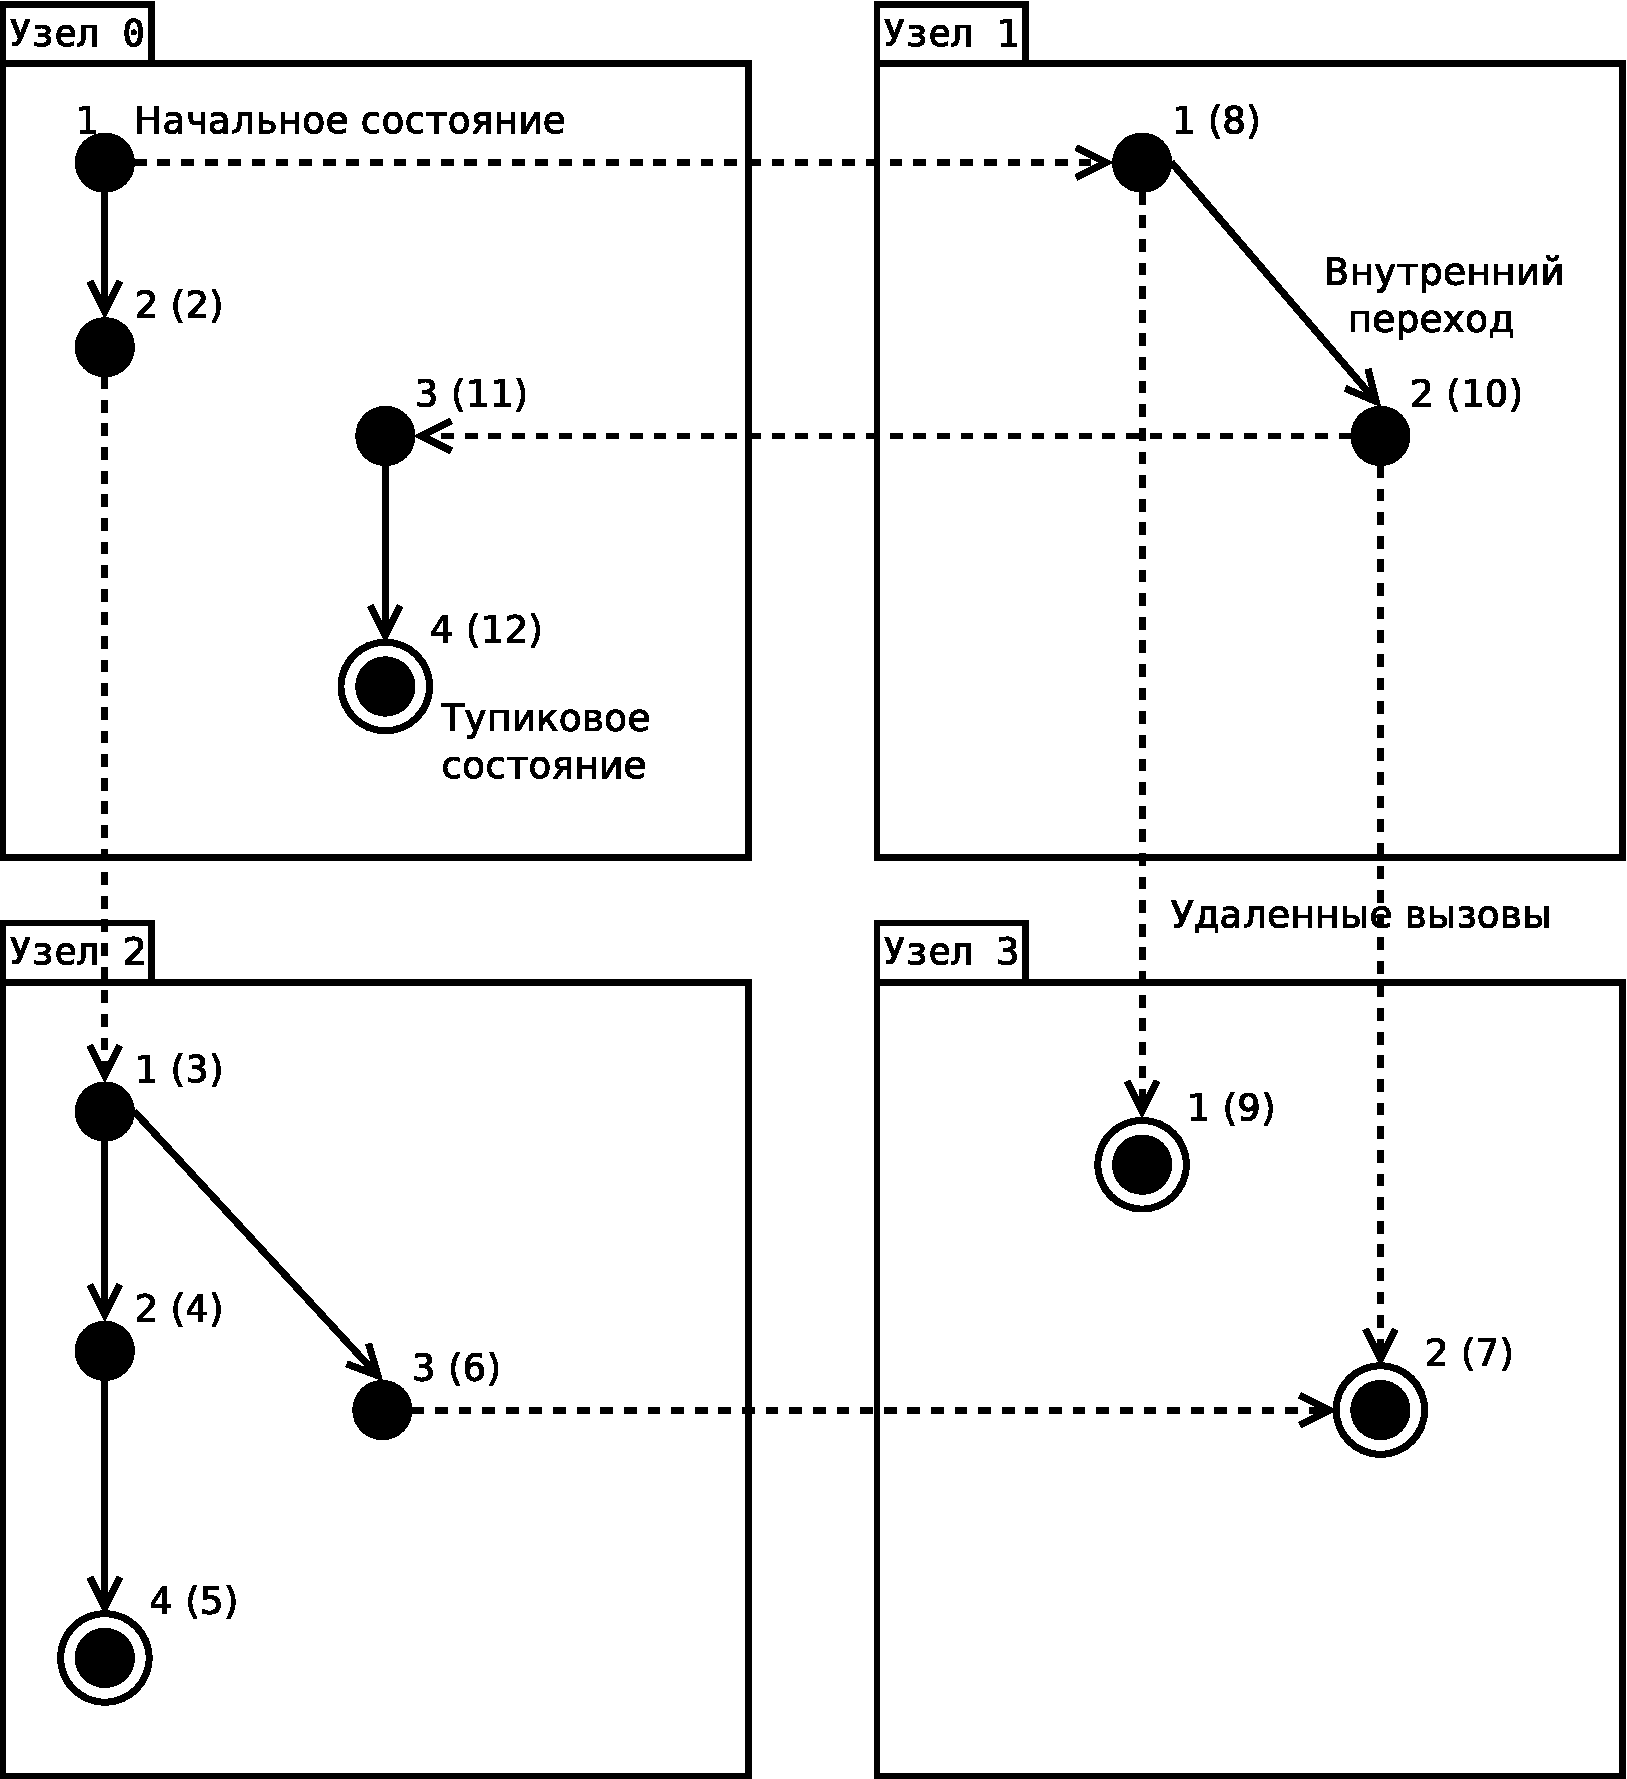
\includegraphics[width=1.0\textwidth]{../graphics/distr-generation}
  \caption{Наглядное представление алгоритма распределенной генерации}
  \label{fig:distr-generation}
\end{figure}

Псевдокод, выполняемый на всех узлах:

\begin{lstlisting}[style=pseudocode]
Visited = ()
Queue   = (initial_state)

def ParStateSpaceBFS():
    while not empty(Queue):
        Queue -> state
        node = StateNode(state)
        if NodeId = node:
            if not state in Visited:
                Visited <- state
                for each new_state in Next(state):
                    Queue <- new_state
        else:
            node.Queue <- state

ParStateSpaceBFS()
\end{lstlisting}

Здесь \Code{node.Queue $\leftarrow$ state}~--- удаленный вызов, добавляющий состояние в очередь узла
\Code{node}.

В отличие от распределенного хранения состояний:
\begin{itemize}
\item удаленные вызовы асинхронные: нет необходимости дожидаться ответа от узла, после
  отправки ему состояния можно продолжать генерацию;
\item возможен (описан далее) подбор такого распределения \Code{StateNode} между узлами,
  при котором число удаленных вызовов будет значительно меньше.~\cite{LS99}
\end{itemize}

Поскольку глобальный порядок обхода состояний нарушается, поиск циклов, необходимый для
проверки условий <<живости>> (см.~раздел~\ref{sec:kripke-verification}) становится
затруднителен. В работах \cite{DLTL1,DLTL2} было предложено несколько различных
алгоритмов, совмещающих приведенный выше поиск в ширину с последующим нахождением циклов
за счет определенной потери производительности, однако они выходят за рамки текущей
работы.

Поскольку нас интересуют лишь условия <<надежности>>, сводимые к проверке утверждений
относительно значений переменных в некоторых состояниях и к проверке финальных
состояний~(\ref{code:philo}), распределенная генерация с поиском в ширину может
использоваться без каких-либо дальнейших модификаций.

\section{Распределение состояний между узлами}
\label{sec:state-partition}

В приведенном коде для определения номера узла, хранящего сообщения, используется функция
\Code{StateNode}. Обязательным требованием к этой функции является зависимость лишь от
самого состояния~--- если два различных узла, $i$ и $j$, сгенерируют одно и то же состояние
$s$, вычисленное на обоих узлах значение \Code{StateNode(s)} должно быть одинаковым.

\paragraph{Равномерность распределения}
\label{sec:partition-homogenity}

Произвольным образом выбранное \Code{StateNode} может привести к тому, что состояния будут
распределены между узлами неравномерно, что приведет к трате памяти на одних узлах и
возможной нехватке на других. Поэтому вторым требованием к \Code{StateNode} является как
можно большая равномерность распределения состояний между узлами. 

Наиболее простым выходом является в качестве \Code{StateNode} использовать хэш-функцию от
всего состояния. Выбор подходящей хэш-функции может обеспечить распределение, близкое к
идеальному.

\paragraph{Локальность распределения}
\label{sec:partition-locality}

Пусть число узлов — $N$, состояний — $S$, переходов между ними — $T$. В случае
равномерного распределения состояний между узлами при помощи хэш-функции вероятность того,
что следующее состояние будет принадлежать текущему узлу равняется
$\frac{1}{N}$. Следовательно, вероятность того, что потребуется удаленный вызов, равна $1
- \frac{1}{N}$, а среднее число удаленных вызовов в течение всей генерации составит
\begin{equation}
  \label{eq:nmsg-full-hash}
  M_1 = T \cdot (1 - \frac{1}{N}) ,
\end{equation}
что при больших значениях $N$ стремится с $T$. Как показывают эксперименты в \cite{LS99},
количество удаленных вызовов является одним из ключевых факторов, определяющих скорость
генерации состояний. Следовательно, третьим желаемым свойством \Code{StateNode} является
локальность получаемого распределения~--- новые состояния должны по возможности
принадлежать тому же узлу, которому принадлежало предыдущее.

Следует отметить, что подобная оптимизация применима лишь при использовании распределенной
генерации, но не распределенного хранилища состояний, описанного в
разделе~\ref{sec:distr-storage}. В последнем случае все состояния генерируются головным
узлом, который может хранить лишь $S/N$ состояний, поэтому вероятность удаленного вызова
при сохранении нового состояния всегда будет не меньше, чем в (\ref{eq:nmsg-full-hash}), и
приближается к $1$ с ростом числа узлов.

В данной работе предлагаются распределение состояний, обладающее свойством
локальности. Оно заключается в том, чтобы хэшировать не все состояние $s$, а состояние
(локальные переменные и $IP$) первых $\rho$ процессов $s$.

Пусть $P$ — число процессов в модели, $k$ — среднее число процессов, затрагиваемых
переходом (состояние которых меняется при переходе). $k > 1$, если возможна (атомарная)
передача сообщений между процессами, при которой сообщение меняют одновременно 2
процесса. $k < 2$, если в одном изменении состояния могут участвовать максимум 2 процесса,
как в языке Promela.

Если предположить, что каждый процесс участвует примерно в равной доле переходов, то для
произвольного наперед заданного процесса вероятность участия в данном переходе составит
$\frac{k}{P}$, а вероятность участия одного из первых $\rho$ процессов~--- $\frac{\rho\cdot
  k}{P}$. Если \Code{StateNode} отображает множество локальных состояний первых $\rho$
процессов на множество узлов равномерным образом, то, по аналогии с предыдущими
рассуждениями, вероятность удаленного вызова при изменении состояния процесса составит $1
- \frac{1}{N}$. Количество удаленных вызовов во всей модели, таким образом, равняется
\begin{equation}
  \label{eq:nmsg-firstproc-hash}
  M_2 = T \cdot \frac{k\cdot\rho}{P} \cdot (1 - \frac{1}{N})
\end{equation}
и с ростом $N$ стремится к $T \cdot \frac{k\rho}{P}$. При количестве процессов $P = 6-8$,
$\rho = 1$ и $k = 1.5$, т.е. когда половина переходов приходится на взаимодействия
процессов, получаем в $P/k = 4-5$ раз меньше удаленных вызовов, чем при хэшировании
состояния целиком.

Значение $\rho$ следует выбирать из баланса между равномерностью распределения состояний и
уменьшением числа удаленных вызовов: если число узлов $N$ достаточно велико, при малых
$\rho$ распределение скорее всего будет неравномерным, а при больших число удаленных
вызовов будет близко к~(\ref{eq:nmsg-full-hash}).

Обозначим $\Omega_i$ число возможных состояний (т.е. всех возможных комбинаций значений
локальных переменных и $IP$) процесса $P_i$. Тогда минимальное значение $\rho$ должно
выбираться таким, чтобы
\begin{equation}
  \label{eq:min-rho}
  \prod_{i = 1}^\rho{\Omega_i} \geq N,
\end{equation}
иначе число возможных значений \Code{StateNode} будет меньше $N$. Если все процессы
одинаковы (или приблизительно одинаковы) и имеют $\Omega$ состояний,~(\ref{eq:min-rho})
превращается в 
\begin{equation}
  \label{eq:min-rho-homo}
  \Omega^\rho \geq N.
\end{equation}

Следует отметить, что, поскольку $IP_i$ входит в \Code{StateNode}, $\Omega_i$ для типичной
модели не меньше 30-40, поэтому $\rho = 1$ может быть достаточно для необходимой
равномерности распределения (обусловленной имеющимся количеством узлов и объемом памяти на
них).

\paragraph{Выбор функции хэширования для распределения состояний}
\label{sec:partition-hash-function}

Хэш-функция $hash_p$, используемая для вычисления \Code{StateNode}, не должна совпадать ни
с одной из функций $hash_i$, используемых для вычисления индекса состояний в
хэш-таблице. 

Допустим, есть состояния $s_1$ и $s_2$ с совпадающими значениями $hash_i(s_1) =
hash_i(s_2)$. Тогда, если $hash_p \equiv hash_j$ при некотором $j$ и, следовательно,
$hash_p(s_1) = hash_p(s_2)$, то оба состояния будут принадлежать одному узлу и при
сохранении их в хэш-таблицу этого узла возникнет коллизия. В то же время, если $hash_p$ не
совпадает ни с одним из $hash_i$, вероятность того, что $s_1$ и $s_2$ будут принадлежать
одному и тому же узлу, составляет лишь $1/N$. Следовательно, использование в качестве
$hash_p$ одной из $hash_i$ повышает частоту коллизий в среднем в $N$ раз.

\section{Экспериментальная проверка распределения}
\label{sec:paremu-test}

Для проверки приведенных выше расчетов был создан прототип системы, имитирующий
параллельную генерацию состояний с распределенным хранением
(см.~раздел~\ref{sec:par-algo}). Данный прототип состоит из транслятора, разбирающего
модель на языке Promela, и генератора состояний на языке~С (подробнее описаны далее в
разделе~\ref{sec:idef0-codegen}).

В качестве модели использовалась приведенная в разделе~\ref{sec:promela} модель задачи об
обедающих философов для случаев $P = 5, 6\text{~и~}7$ (количество процессов совпадает с
количеством философов). В качестве \Code{NodeState} используются оба рассмотренных ранее
варианта: хэш-функция от всего состояния и от состояния первого процесса ($\rho = 1$).

Результаты экспериментов для имитации ЛВС из 4 узлов представлены в
табл.~\ref{tab:paremu-stats}. В столбцах <<Состояния>> и <<Переходы>> указано общее число
состояний и переходов модели. В столбце <<Удаленные вызовы>>~--- число (суммарное по всем
узлам) удаленных вызовов за время имитации: слева~--- при использовани хэш-функции от
всего состояния, справа~--- от состояния одного процесса. В столбце <<Загруженность
узлов>> в качестве меры <<равномерности>> распределения состояний между узлами показано
отношение минимального и максимального объема используемой памяти среди всех узлов.

\begin{table}[ht]
  \centering
  \begin{tabular}[ht]{|r|c|c|c|c|c|c|}
    \hline
    P & Состояния & Переходы & \multicolumn{2}{|c|}{Сообщения} & \multicolumn{2}{|c|}{Равномерность}    \\
    \hline
    5 & 28351     & 42658    & 31356  (73\%) & 7047  (16\%) & 0.99 & 0.66 \\ 
    6 & 147774    & 232748   & 170378 (73\%) & 31668 (13\%) & 0.99 & 0.68 \\ 
    7 & 360354    & 601462   & 453789 (75\%) & 66438 (11\%) & 0.99 & 0.74 \\ 
    \hline
  \end{tabular}
  \caption{Результаты имитации параллельной генерации}
  \label{tab:paremu-stats}
\end{table}

Из приведенных выше результатов можно сделать следующие выводы:

\begin{enumerate}
\item При использовании в качестве \Code{StateNode} хэша всего состояния число
  удаленных вызовов действительно приближается к числу всех переходов, как и
  следует из (\ref{eq:nmsg-full-hash}).

\item Использование вместо нее хэша от состояния только одного (первого) процесса приводит
  к сокращению числа удаленных вызовов, которое довольно точно оценивается
  формулой~(\ref{eq:nmsg-firstproc-hash}).

\item Равномерность распределения состояний между узлами падает в последнем
  случае, что приводит к простою части памяти  (до 30\% на некоторых узлах),
  поэтому возможно дальнейшее улучшение функции распределения.
\end{enumerate}

%%% Local Variables: 
%%% mode: latex
%%% TeX-master: "thesis"
%%% End: 
